\chapter{Návrh systému}
\label{kap_navrh_systemu}
V předchozích dvou kapitolách byla rozebrána teoretická část problému. V této kapitole shrneme požadavky vyplývající z teorie, které je nutno zakomponovat do
výsledného systému. Nejprve bude schématicky vyjádřena obecná funkcionalita systému, která se následně bude rozebírat detailněji.

\section{Teoretické požadavky}
Nároky na systém, které vyplývají z teorie můžeme rozdělit do tří částí - implementace SNMP protokolu, implementace navrženého XML protokolu a propojení těchto dvou protokolů dohromady.

Hlavním požadavkem, který vyplývá i ze zadání práce, je vytvořit modulární systém, který bude nejenom spojovat současné verze protokolů, ale bude počítat i s potenciálním rozšířením do
budoucna. Obecné schéma navrhovaného systému zobrazuje obrázek \ref{obr_an_obecne_schema}. 

\begin{figure}[htp]
	\begin{center}
		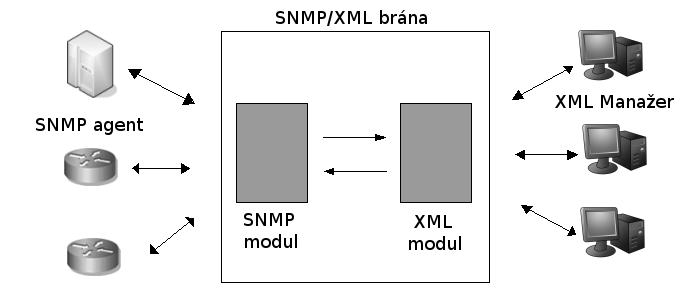
\includegraphics[width=15cm]{obrazky/04_obecne_schema.png}
		\caption{Schéma navrhovaného systému}
		\label{obr_an_obecne_schema}
	\end{center}
\end{figure}

Zde je vidět, že oba dva protokolové moduly jsou na sobě nezávislé a jejich interakce spočívá v předávání si zpráv. Nyní přejděme k detailnějším požadavkům na výše zmíněné části systému.

V rámci \textit{SNMP protokolu} je požadováno
\begin{itemize}
	\item implementace komunikačních struktur protokolů SNMPv1 a SNMPv2
	\item převzetí bezpečnostního schématu z tohoto protokolu
\end{itemize}

\textit{XML orientovaná část programu } má za úkol
\begin{itemize}
	\item implementovat komunikační struktury navrženého protokolu
	\item navrhnout efektivní správu XML struktur v paměti
	\item poskytnout XML manažerům transparentní získání dat z monitorovaných zařízení
	\item mapovat rozšířenou množinu funkcí v rámci XML protokolu do SNMP
	\item s manažery komunikovat pouze přes HTTP/HTTPS protokol
\end{itemize}
Spojením protokolů je myšlen přechod od databázových struktur jednoho protokolu k druhému. V našem případě je to transformace SNMP MIB do XML, jak bylo vysvětleno v kapitole \ref{kap_xml}.

\subsection{XML}
Nejprve se zaměříme na reprezentaci dat, které budou v rámci XML popisovat jak bránu, tak monitorované zařízení. Z předchozích kapitol vyplynulo, že bude použito částečně objektového přístupu a přímého mapování MIB.
Strukturu dat bude popisovat XML dokument, strom, který má strukturu vyjádřenou na obrázku \ref{obr_an_strom_struktura}.

\begin{figure}[htp]
	\begin{center}
		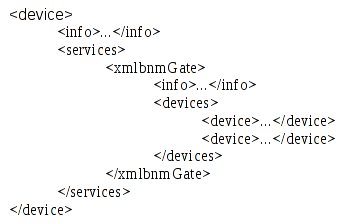
\includegraphics{obrazky/04_schema_dokumentu.png}
		\caption{Obecná struktura XML dokumentu}
		\label{obr_an_strom_struktura}
	\end{center}
\end{figure}

\begin{figure}[htp]
	\begin{center}
		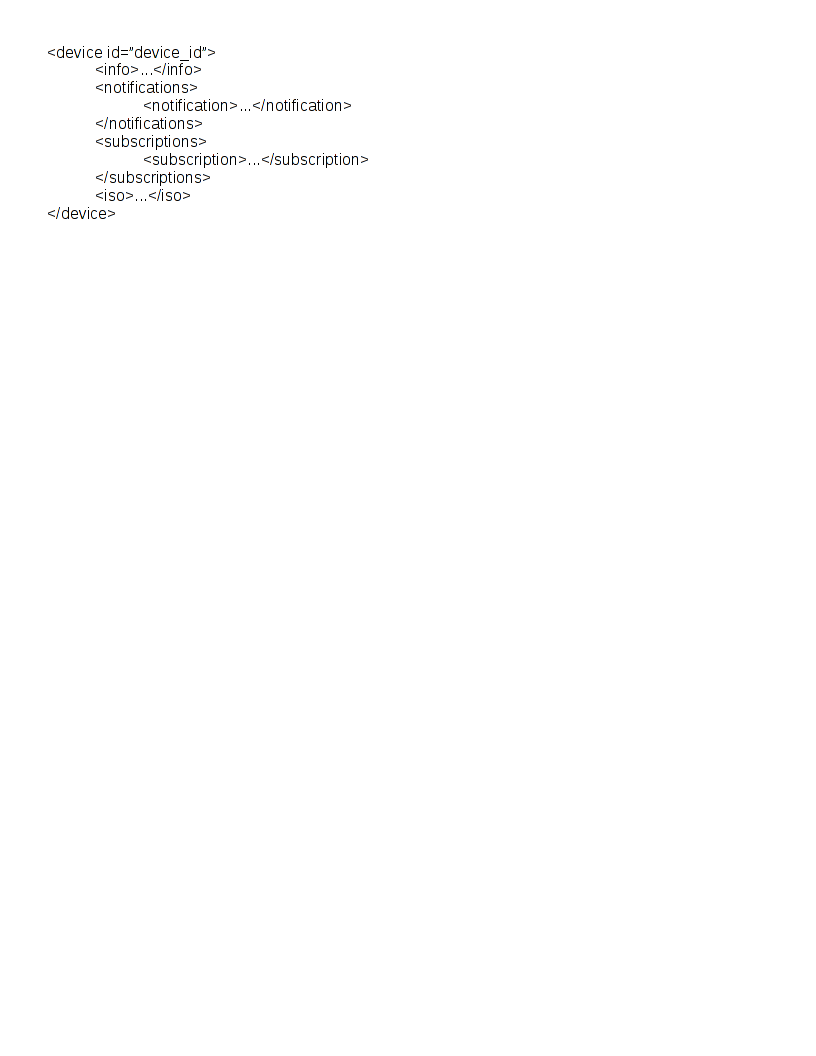
\includegraphics{obrazky/04_schema_device.png}
		\caption{Struktura elementu device}
		\label{obr_an_device_struktura}
	\end{center}
\end{figure}

Kořenový uzel specifikuje celé zařízení vystupující jako protokolová brána, obsahuje tyto elementy:
\begin{itemize}
	\item \textbf{info} - tento element obsahuje text, kterým je popsáno dané zařízení
	\item \textbf{services} - element vymezující poskytované služby (při širší implementaci může obsahovat služby DNS, DHCP, apod.)
	\item \textbf{xmlbnmGate} - naše služba poskytující spojení XML a SNMP protokolu
	\item \textbf{device} - je podelementem \textbf{xmlbnmGate} a vymezuje jedno monitorované zařízení
\end{itemize}

Prvky \textbf{device} jsou do XML dokumentu přidávány na základě informací v konfiguračním souboru (viz kapitola \ref{sec_an_struktura_programu}).

Strukturu elementu \textbf{device} popisuje obrázek \ref{obr_an_device_struktura}. Každý takovýto element bude obsahovat následující informace:
\begin{itemize}
	\item \textbf{info} - stejně jako kořenový element popisuje dané zařízení
	\item \textbf{notifications} - obsahuje elementy a typy upozornění (TRAP zprávy v rámci SNMP), na které manažer čeká
	\item \textbf{subscriptions} - obsahuje informace o datech, které si nechává manažer posílat v pravidelných intervalech (více v popisu komunikace)
	\item \textbf{data} - dětmi tohoto elementu jsou veškerá data přímo z MIB.
\end{itemize}

Samotný element má atribut \textit{id}, což je jeho identifikace v rámci xml dokumentu. Dle tohoto unikátního čísla je pak možné
v sadě dotazů rozpoznat, ke kterému zařízení se dotaz vztahuje.

Element \textbf{info} obsahuje elementy, které specifikují jméno a popis zařízení (viz obrázek \ref{obr_an_info_element}).

\begin{figure}[htp]
	\begin{center}
		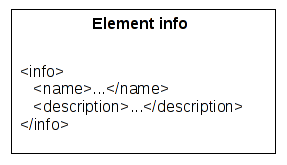
\includegraphics{obrazky/04_element_info.png}
		\caption{Struktura elementu info}
		\label{obr_an_info_element}
	\end{center}
\end{figure}

Jednotlivé podelementy uzlu \textbf{subscriptions} musí z podstaty věci obsahovat informace, které určují, jaké objekty chce manažer pravidelně sledovat, identifikovat
manažera, aby mu mohla být data doručena a specifikovat časový interval, tj. frekvenci sledování příslušné veličiny.

Potomci uzlu \textbf{notifications} určují, které typy událostí jsou sledovány u daného zařízení. V rámci konfigurace systému je nezbytné, aby pro každé zařízení
bylo jasně definováno, kam mají být příslušné zprávy o událostech zasílány. Tato informace bude součástí konfiguračního souboru a systém ji bude
interně zpracovávat. Samotný XML tag bude obsahovat unikátní identifikační číslo (OID) dané události, aby jej bylo možno poté identifikovat a správně formulovat
XML zprávu manažerovi.

Mapování dat z MIB bylo obecně popsáno v kapitole \ref{kap_xml} a přesný algoritmus bude specifikován v následující kapitole. Pro adresaci jednotlivých objektů
je, jak bylo již nastíněno v předchozí kapitole, použito mechanismů XPath či XQuery. Dotaz na položku z MIB může vypadat následovně
\begin{verbatim}
	/iso/org/dod/internet/mgmt/mib-2/...
\end{verbatim}

Důležitým faktem je, že manažer se ptá přímo na uzly datového stromu. Nemusí tedy uvádět cestu v rámci celého stromu, který popisuje strukturu brány.

\subsubsection*{Zprávy}
Zprávy, které budou posílány mezi manažerem a bránou, mají formu XML dokumentu. Schématicky je znázorněna a popsána v kapitole \ref{kap_xml}, obrázek \ref{obr_xml_struktura_zpravy}.

Kořenový element message obaluje veškerá posílaná data. Může obsahovat několik dílčích dotazů, nastavení a ostatních informací, které budou vykonávány postupně
jedna po druhé. V rámci teorie byla nastíněna možnost použití několika různých front, které by byly specifikovány identifikátorem a zaručovaly by různou
prioritu zpracování. Navrhovaný systém bude podporovat rozdělení komunikačních front dle monitorovaných zařízení. Zajistí se tím správné pořadí vykonání
příchozích požadavků.

Komunikace mezi manažerem a bránou je na XML úrovni omezena na zprávy
\begin{itemize}
	\item Get
	\item Set
	\item Discovery
	\item Publication
	\item Subscription
	\item Distribution
	\item Event
\end{itemize}

Přesná struktura a popis funkce jednotlivých zpráv byla popsána v předchozí kapitole.


\subsubsection*{Komunikační protokol}
Od protokolu SNMP se XML část komunikace liší také tím, že bude probíhat na spolehlivém a potvrzovaném protokolu - HTTP. Každá zpráva, která
je poslána, musí mít potvrzeno doručení, což tento aplikační protokol, využívající transportního protokolu TCP, nabízí. 

Informace budou posílány ve formátu HTTP POST zprávy. Strukturu dotazu a odpovědi zobrazuje obrázek \ref{obr_an_http_post} a komunikaci obrázek \ref{obr_an_http_request}.

\begin{figure}[htp]
	\begin{center}
		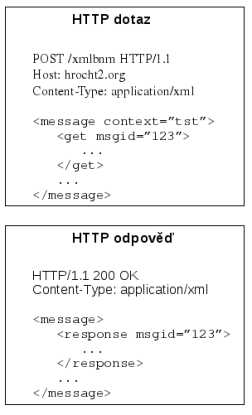
\includegraphics{obrazky/04_http_post.png}
		\caption{HTTP zprávy předávané mezi manažerem a bránou}
		\label{obr_an_http_post}
	\end{center}
\end{figure}

\begin{figure}[htp]
	\begin{center}
		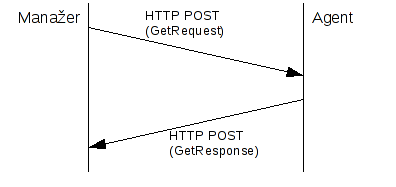
\includegraphics{obrazky/04_http_request.png}
		\caption{HTTP komunikace mezi manažerem a agentem/bránou}
		\label{obr_an_http_request}
	\end{center}
\end{figure}

Otázka bezpečného přenosu dat byla řešena v předchozí kapitole a byl zvolen protokol HTTPS. Zajištění distribuce a zpracování certifikátů bude
diskutováno dále v této kapitole.


\subsection{SNMP}
Druhou část komunikace tvoří SNMP protokol. Z kapitoly \ref{kap_snmp} vychází seznam zpráv, které je nutné implementovat:
\begin{itemize}
	\item Get
	\item Set
	\item Response
	\item GetNext
	\item Trap
\end{itemize}

V rámci komunikace se v této práci budeme zaobírat verzemi SNMPv1 a SNMPv2. Samotná implementace a mapování SNMP zpráv na XML dotazy
bude diskutována až v kapitole \ref{kap_implementace}.

Bezpečnost se v SNMP omezuje pouze na komunitní heslo. V rámci XML protokolu je bezpečnost založena jednak na šifrovaném přenosu dat mezi
manažerem a bránou, druhak na přístupovém heslu, které vymezuje čtecí či zápisová práva při přístupu k zařízení. 


\section{Struktura programu}
\label{sec_an_struktura_programu}
Před samotným návrhem jednotlivých funkčních elementů je nutno zvolit, jak bude program fungovat a jevit se globálně. Vzhledem k
nabízeným službám a komunikaci je možné zvolit koncepci podobnou webovým službám (založených na principu SOAP). Druhým možným přístupem je zvolit
na pozadí běžící aplikaci - démona, který bude po celou dobu svého běhu monitorovat a zpracovávat příchozí požadavky.

\subsection{SOAP vs. démon}
Kompozice struktury jako webové služby založené na SOAP architektuře má několik předností. Je tím hlavně přenositelnost a jednoduchost nasazení. Vše, co je potřeba k běhu,
je aplikační server. Nainstalování a spuštění služby je již pak otázkou okamžiku. Samotná struktura kódu je též o něco jednodušší než v případě démona. Je nutné se starat pouze o
příchozí požadavek a jeho zpracování.

Bohužel tento přístup má ale i mnoho nevýhod. Zaprvé je to reakční doba, za kterou je systém schopen zaslat manažerovi odpověď. Pro samotné zpracování požadavku
je nutno v paměti (či v souboru) udržovat XML reprezentaci MIB tak, jak bylo popsáno dříve. Při použití tohoto postupu se po každém přijatém požadavku musí načíst informace ze souboru
a teprve poté je možno data zpracovat.

Dalším sporným bodem je periodické zasílání zpráv manažerům, kteří o to požádali zprávou Subscription. V takovém případě musí běžet jeden proces, který v určených intervalech zasílá SNMP
dotazy na monitorované zařízení, což je neslučitelné se základní myšlenkou webových služeb.

Asi největší nevýhodou tohoto přístupu je transformace dat z MIB do XML. Při spuštění webové služby je nutné, aby všechna zařízení již měla své monitorované informace uloženy v XML formátu, 
protože při požadavku již není čas data transformovat. Tento akt by musel být od služby oddělen a buď svěřen periodicky se spouštěnému skriptu, nebo by jej administrátor musel provést pokaždé,
když se změní počet, druh či monitorované údaje jednotlivých zařízení.

Oproti tomu stojí druhý přístup - strukturovat aplikaci jako démona. Je pravdou, že výsledný kód aplikace je složitější, přenositelnost horší a není zde možné mluvit o platformové nezávislosti (co se implementace v C++ týče).
Nicméně získáme tím výhodu v podobě relativně malé reakční doby, protože veškeré informace jsou za běhu uloženy v operační paměti a není je nutno načítat z pevného disku. Systém periodického monitorování
zařízení může být jednoduše spravován jedním vláknem procesu, zatímco ostatní vlákna se starají o příchozí a odchozí požadavky. Transformace dat pak může být bez úhony součástí samotného programu.

\subsection{Navrhovaná aplikace}
Fáze běhu navrhovaného systému zobrazuje diagram na obrázku \ref{obr_an_beh_programu}.

\begin{figure}[htp]
	\begin{center}
		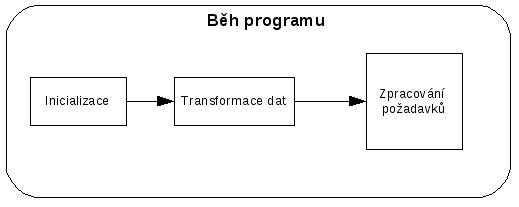
\includegraphics{obrazky/04_beh_programu.png}
		\caption{Fáze běhu programu}
		\label{obr_an_beh_programu}
	\end{center}
\end{figure}

\subsubsection{Inicializace}
V první, inicializační, fázi je načten konfigurační soubor, jehož specifikace bude popsána v kapitole \ref{kap_implementace}. Tento soubor obsahuje veškeré informace o monitorovaných zařízeních, stejně tak
jako základní nastavení protokolové brány. Každé zařízení musí mít definováno SNMP spojení (adresu), seznam MIB, které vyjadřují všechny nabízené informace. Dále bude obsahovat nastavení ohledně 
asynchronních událostí a jakému manažerovi je nutno je přeposílat. Důležitým nastavením je i verze SNMP protokolu, jakou zařízení podporuje.

Protokolová brána bude mít sama o sobě speciální část, která bude definovat komunikační porty, na kterých budou přijímány a zpracovávány požadavky, cesty k různým logovacím souborům a cesty k adresáři s MIB a XML soubory.

Součástí inicializace je i ověření, zda-li všechna monitorovaná zařízení fungují. Pakliže některé nebudou funkční, systém je ze seznamu vyškrtne a nebude je nabízet manažerům ke správě.

\subsubsection{Transformace dat}
Transformace dat představuje samotné mapování MIB do XML tak, jak bylo popsáno dříve. Pro každé zařízení může být specifikováno několik různých MIB, jak veřejné, tak proprietární. Pro každé
zařízení je tedy nutno vytvořit XML dokument, popisující veškeré MIB informace.

V tomt místě jsou možné dvě cesty, jak vybudovat výstupní XML dokument. Jednou možností je zahrnout veškeré informace o všech zařízeních do jednoho souboru, který potom bude rozesílán každému manažerovi, jenž si o něj řekne. Tato varianta
je sice praktická, ale neefektivní. Pro zařízení s velkým množstvím informací by byl výsledný dokument opravdu veliký. Kdyby manažer chtěl spravovat pouze jediné zařízení, byl by stejně nucen stáhnout velký objem dat, než
by mu bylo dovoleno pracovat dále.

Proto bude použito následujícího schématu. Systém bude při prvním kontaktu s manažerem publikovat pouze informace týkající se počtu a typu zařízení, které spravuje. Jednotlivá zařízení budou mít svůj samostatný soubor
s daty. Manažer si pak bude moci zvolit pouze určitá data, která ho zajímají. Tím se velmi sníží počáteční zatížení linky.

\subsubsection{Zpracovávání požadavků}
Po úspěšném průchodu oběma předchozími fázemi se program dostává do situace, kdy vyčkává na příchozí požadavky, ať již ze strany manažerai, či SNMP zařízení.

Jak již bylo popsáno na začátku této kapitoly, o komunikaci se starají dva moduly - SNMP a XML. Proto taky komunikační rozhraní se dělí na dvě části.

SNMP modul bude komunikovat pomocí protokolu UDP, posíláním SNMP zpráv. Tato část rozhraní bude blíže popsána v následující kapitole.

Komunikace v rámci XML je na bázi HTTP protokolu. Pro zpracování mnoha požadavků, které je nutno očekávat, bude použito HTTP serveru. V tomto případě se nám nabízí dvě možnosti
řešení - využijeme nějakého již stávajícího webového serveru (Apache, Tomcat, ...), na kterém budeme spouštět CGI script a tak komunikovat s naším programem, nebo do aplikace nějaký jednoduchý server
naimplementujeme. Výhodou již existujícího řešení by byla pouhá konstrukce komunikačního kanálu mezi protokolovou branou a zmíněným serverem. Je ale pravděpodobné, že bude potřeba mít větší kontrolu
nad přijímanými a odesílanými zprávami, což vlastní implementovaný server poskytuje. Přednostně tedy bude vybrána varianta s embedded HTTP serverem.

Ve spojitosti s protokolem HTTP je nutné zmínit použití certifikátů pro zabezpečený přenost a použití protokolu HTTPS. Kdyby bylo využito externího webového serveru, bude ponechána
veškerá zodpovědnost a konfigurace na administrátorovi serveru, který se bude muset postarat o obdržení a distribuci certifikátu. Jestli bude server součástí protokolové brány, bude
nutno přiložit certifikát k aplikaci a v konfiguračním souboru zajistit jeho použití.

\section{Správa protokolové brány}
V rámci spravovaných zařízení se naskýtá otázka, jestli by bylo možno spravovat i samotnou bránu přes navržený XML protokol (je myšlena aplikace jako taková). 

Navržený systém tuto skutečnost neumožňuje. Samotná brána nebude vykazovat vlastnosti agenta. Ke správě stroje, na kterém brána poběží, bude nutné použít XML či SNMP agenta, který tuto 
funkcionalitu bude zajišťovat. Je možné pak v konfiguračním souboru nastavit, aby brána nabízela komunikaci se SNMP agentem na tomtéž stroji. XML agent bude komunikovat s manažerem přímo na definovaném portu.
Implementace takového agenta ale již přesahuje rámec této práce.

Správa aplikace je pak omezena pouze na konfigurační soubor a bude ji nutné při každé změně restartovat (jak je tomu například i u konfigurace webových serverů). Je to z důvodu zachování integrity poskytovaných dat.
Při změně informačních bází jednotlivých zařízení, přidání či odebrání monitorovaných strojů, je nutno přegenerovat všechny XML dokumenty, které jsou pak distribuovány manažerům. Nekorektnost dat, které manažer obdržel a které
by byly aktuální, kdyby se změnily za plného provozu, by mohla mít pak vážné následky na data, která by manažeři dostali zpět.

\section{XML manažerská aplikace}
Součástí této práce je i implementace základního XML manažera tak, aby dovolil ukázat veškeré funkční aspekty protokolové brány.

Program bude mít implementován celý XML komunikační protokol tak, jak byl navržen v kapitole \ref{kap_xml}. Bude podporovat základní příkazy - Discovery, Publication, Get, Set, Subscription, Distribution.

Správu monitorovaných zařízení zahajuje komunikací buď přímo s agentem či bránou. Vyžádá si od nich 
dokument, který popisuje nabízené informace. Pakliže se jedná o komunikaci s bránou, tak nejprve zjistí, jaká zařízení jsou k dispozici a pak si některé vybere a teprve pak požádá o jejich XML popis dat.
Algoritmus budování XML stromu použitelného pro další interakci se zařízeními je stejný jako v případě brány a bude popsán v další kapitole. 

Aplikace bude napsána v jazyce C++ stejně jako protokolová brána. Využití podpory grafického rozhraní je možné.







